\documentclass[10pt,t,aspectratio=43,handout]{beamer} % handout aspectratio=149,1610,32,54
\usetheme{Heverlee}
\usepackage{amsmath,amssymb}
\usepackage{tikz-cd,tikz}
\usepackage{mathtools,mathbbol}
\usepackage{subcaption}
\usepackage{algorithm2e}

% environments
%\newtheorem{theorem}{Theorem}
\newtheorem*{theorem*}{Theorem}
\newtheorem{proposition}[theorem]{Proposition}
\newtheorem*{proposition*}{Proposition}
%\newtheorem{lemma}[theorem]{Lemma}
\newtheorem*{lemma*}{Lemma}
%\newtheorem{corollary}[theorem]{Corollary}
\newtheorem*{corollary*}{Corollary}

\theoremstyle{definition}
%\newtheorem{definition}[theorem]{Definition}
\newtheorem*{definition*}{Definition}
\newtheorem{remark}[theorem]{Remark}
\newtheorem*{remark*}{Remark}
%\newtheorem{example}[theorem]{Example}
\newtheorem*{example*}{Example}
\newtheorem{construction}[theorem]{Construction}
\newtheorem*{construction*}{Construction}
\newtheorem{convention}[theorem]{Convention}
\newtheorem*{convention*}{Convention}
\newtheorem{terminology}[theorem]{Terminology}
\newtheorem*{terminology*}{Terminology}
\newtheorem{notation}[theorem]{Notation}
\newtheorem*{notation*}{Notation}
\newtheorem{question}[theorem]{Question}
\newtheorem*{question*}{Question}

% hyphenation
\hyphenation{co-chain}
\hyphenation{co-chains}
\hyphenation{co-al-ge-bra}
\hyphenation{co-al-ge-bras}
\hyphenation{co-bound-ary}
\hyphenation{co-bound-aries}
\hyphenation{Func-to-rial-i-ty}
\hyphenation{colim-it}
\hyphenation{di-men-sional}

% basics
\DeclareMathOperator{\face}{d}
\DeclareMathOperator{\dege}{s}
\DeclareMathOperator{\bd}{\partial}
\DeclareMathOperator{\sign}{sign}
\newcommand{\ot}{\otimes}
\DeclareMathOperator{\EZ}{EZ}
\DeclareMathOperator{\AW}{AW}

% sets and spaces
\newcommand{\N}{\mathbb{N}}
\newcommand{\Z}{\mathbb{Z}}
\newcommand{\Q}{\mathbb{Q}}
\newcommand{\R}{\mathbb{R}}
\renewcommand{\k}{\Bbbk}
\newcommand{\sym}{\mathbb{S}}
\newcommand{\cyc}{\mathbb{C}}
\newcommand{\Ftwo}{{\mathbb{F}_2}}
\newcommand{\Fp}{{\mathbb{F}_p}}
\newcommand{\Cp}{{\cyc_p}}
\newcommand{\gsimplex}{\mathbb{\Delta}}
\newcommand{\gcube}{\mathbb{I}}

% categories
\newcommand{\Cat}{\mathsf{Cat}}
\newcommand{\Fun}{\mathsf{Fun}}
\newcommand{\Set}{\mathsf{Set}}
\newcommand{\Top}{\mathsf{Top}}
\newcommand{\CW}{\mathsf{CW}}
\newcommand{\Ch}{\mathsf{Ch}}
\newcommand{\simplex}{\triangle}
\newcommand{\sSet}{\mathsf{sSet}}
\newcommand{\cube}{\square}
\newcommand{\cSet}{\mathsf{cSet}}
\newcommand{\Alg}{\mathsf{Alg}}
\newcommand{\coAlg}{\mathsf{coAlg}}
\newcommand{\biAlg}{\mathsf{biAlg}}
\newcommand{\sGrp}{\mathsf{sGrp}}
\newcommand{\Mon}{\mathsf{Mon}}
\newcommand{\symMod}{\mathsf{Mod}_{\sym}}
\newcommand{\symBimod}{\mathsf{biMod}_{\sym}}
\newcommand{\operads}{\mathsf{Oper}}
\newcommand{\props}{\mathsf{Prop}}

% operators
\DeclareMathOperator{\free}{F}
\DeclareMathOperator{\forget}{U}
\DeclareMathOperator{\yoneda}{\mathcal{Y}}
\DeclareMathOperator{\Sing}{Sing}
\newcommand{\loops}{\Omega}
\DeclareMathOperator{\cobar}{\mathbf{\Omega}}
\DeclareMathOperator{\proj}{\pi}
\DeclareMathOperator{\incl}{\iota}
\DeclareMathOperator{\Sq}{Sq}
\DeclareMathOperator{\ind}{ind}
\DeclareMathOperator{\rank}{rank}

% chains
\DeclareMathOperator{\chains}{N}
\DeclareMathOperator{\cochains}{N^{\vee}}
\DeclareMathOperator{\gchains}{C}

% pair delimiters (mathtools)
\DeclarePairedDelimiter\bars{\lvert}{\rvert}
\DeclarePairedDelimiter\norm{\lVert}{\rVert}
\DeclarePairedDelimiter\angles{\langle}{\rangle}
\DeclarePairedDelimiter\set{\{}{\}}
\DeclarePairedDelimiter\ceil{\lceil}{\rceil}
\DeclarePairedDelimiter\floor{\lfloor}{\rfloor}

% other
\newcommand{\id}{\mathsf{id}}
\renewcommand{\th}{\mathrm{th}}
\newcommand{\op}{\mathrm{op}}
\DeclareMathOperator*{\colim}{colim}
\DeclareMathOperator{\coker}{coker}
\newcommand{\Hom}{\mathrm{Hom}}
\newcommand{\End}{\mathrm{End}}
\newcommand{\coEnd}{\mathrm{coEnd}}
\newcommand{\xla}[1]{\xleftarrow{#1}}
\newcommand{\xra}[1]{\xrightarrow{#1}}
\newcommand{\defeq}{\stackrel{\mathrm{def}}{=}}

% comments
\newcommand{\anibal}[1]{\noindent\textcolor{blue}{\underline{Anibal}: #1}}

% pdf
\newcommand{\pdfEinfty}{\texorpdfstring{${E_\infty}$}{E-infty}}

% mathrm
\newcommand{\rA}{\mathrm{A}}
\newcommand{\rB}{\mathrm{B}}
\newcommand{\rC}{\mathrm{C}}
\newcommand{\rD}{\mathrm{D}}
\newcommand{\rE}{\mathrm{E}}
\newcommand{\rF}{\mathrm{F}}
\newcommand{\rG}{\mathrm{G}}
\newcommand{\rH}{\mathrm{H}}
\newcommand{\rI}{\mathrm{I}}
\newcommand{\rJ}{\mathrm{J}}
\newcommand{\rK}{\mathrm{K}}
\newcommand{\rL}{\mathrm{L}}
\newcommand{\rM}{\mathrm{M}}
\newcommand{\rN}{\mathrm{N}}
\newcommand{\rO}{\mathrm{O}}
\newcommand{\rP}{\mathrm{P}}
\newcommand{\rQ}{\mathrm{Q}}
\newcommand{\rR}{\mathrm{R}}
\newcommand{\rS}{\mathrm{S}}
\newcommand{\rT}{\mathrm{T}}
\newcommand{\rU}{\mathrm{U}}
\newcommand{\rV}{\mathrm{V}}
\newcommand{\rW}{\mathrm{W}}
\newcommand{\rX}{\mathrm{X}}
\newcommand{\rY}{\mathrm{Y}}
\newcommand{\rZ}{\mathrm{Z}}
% mathcal
\newcommand{\cA}{\mathcal{A}}
\newcommand{\cB}{\mathcal{B}}
\newcommand{\cC}{\mathcal{C}}
\newcommand{\cD}{\mathcal{D}}
\newcommand{\cE}{\mathcal{E}}
\newcommand{\cF}{\mathcal{F}}
\newcommand{\cG}{\mathcal{G}}
\newcommand{\cH}{\mathcal{H}}
\newcommand{\cI}{\mathcal{I}}
\newcommand{\cJ}{\mathcal{J}}
\newcommand{\cK}{\mathcal{K}}
\newcommand{\cL}{\mathcal{L}}
\newcommand{\cM}{\mathcal{M}}
\newcommand{\cN}{\mathcal{N}}
\newcommand{\cO}{\mathcal{O}}
\newcommand{\cP}{\mathcal{P}}
\newcommand{\cQ}{\mathcal{Q}}
\newcommand{\cR}{\mathcal{R}}
\newcommand{\cS}{\mathcal{S}}
\newcommand{\cT}{\mathcal{T}}
\newcommand{\cU}{\mathcal{U}}
\newcommand{\cV}{\mathcal{V}}
\newcommand{\cW}{\mathcal{W}}
\newcommand{\cX}{\mathcal{X}}
\newcommand{\cY}{\mathcal{Y}}
\newcommand{\cZ}{\mathcal{Z}}
% mathsf
\newcommand{\sA}{\mathsf{A}}
\newcommand{\sB}{\mathsf{B}}
\newcommand{\sC}{\mathsf{C}}
\newcommand{\sD}{\mathsf{D}}
\newcommand{\sE}{\mathsf{E}}
\newcommand{\sF}{\mathsf{F}}
\newcommand{\sG}{\mathsf{G}}
\newcommand{\sH}{\mathsf{H}}
\newcommand{\sI}{\mathsf{I}}
\newcommand{\sJ}{\mathsf{J}}
\newcommand{\sK}{\mathsf{K}}
\newcommand{\sL}{\mathsf{L}}
\newcommand{\sM}{\mathsf{M}}
\newcommand{\sN}{\mathsf{N}}
\newcommand{\sO}{\mathsf{O}}
\newcommand{\sP}{\mathsf{P}}
\newcommand{\sQ}{\mathsf{Q}}
\newcommand{\sR}{\mathsf{R}}
\newcommand{\sS}{\mathsf{S}}
\newcommand{\sT}{\mathsf{T}}
\newcommand{\sU}{\mathsf{U}}
\newcommand{\sV}{\mathsf{V}}
\newcommand{\sW}{\mathsf{W}}
\newcommand{\sX}{\mathsf{X}}
\newcommand{\sY}{\mathsf{Y}}
\newcommand{\sZ}{\mathsf{Z}}
% mathbb
\newcommand{\bA}{\mathbb{A}}
\newcommand{\bB}{\mathbb{B}}
\newcommand{\bC}{\mathbb{C}}
\newcommand{\bD}{\mathbb{D}}
\newcommand{\bE}{\mathbb{E}}
\newcommand{\bF}{\mathbb{F}}
\newcommand{\bG}{\mathbb{G}}
\newcommand{\bH}{\mathbb{H}}
\newcommand{\bI}{\mathbb{I}}
\newcommand{\bJ}{\mathbb{J}}
\newcommand{\bK}{\mathbb{K}}
\newcommand{\bL}{\mathbb{L}}
\newcommand{\bM}{\mathbb{M}}
\newcommand{\bN}{\mathbb{N}}
\newcommand{\bO}{\mathbb{O}}
\newcommand{\bP}{\mathbb{P}}
\newcommand{\bQ}{\mathbb{Q}}
\newcommand{\bR}{\mathbb{R}}
\newcommand{\bS}{\mathbb{S}}
\newcommand{\bT}{\mathbb{T}}
\newcommand{\bU}{\mathbb{U}}
\newcommand{\bV}{\mathbb{V}}
\newcommand{\bW}{\mathbb{W}}
\newcommand{\bX}{\mathbb{X}}
\newcommand{\bY}{\mathbb{Y}}
\newcommand{\bZ}{\mathbb{Z}}
% mathfrak
\newcommand{\fA}{\mathfrak{A}}
\newcommand{\fB}{\mathfrak{B}}
\newcommand{\fC}{\mathfrak{C}}
\newcommand{\fD}{\mathfrak{D}}
\newcommand{\fE}{\mathfrak{E}}
\newcommand{\fF}{\mathfrak{F}}
\newcommand{\fG}{\mathfrak{G}}
\newcommand{\fH}{\mathfrak{H}}
\newcommand{\fI}{\mathfrak{I}}
\newcommand{\fJ}{\mathfrak{J}}
\newcommand{\fK}{\mathfrak{K}}
\newcommand{\fL}{\mathfrak{L}}
\newcommand{\fM}{\mathfrak{M}}
\newcommand{\fN}{\mathfrak{N}}
\newcommand{\fO}{\mathfrak{O}}
\newcommand{\fP}{\mathfrak{P}}
\newcommand{\fQ}{\mathfrak{Q}}
\newcommand{\fR}{\mathfrak{R}}
\newcommand{\fS}{\mathfrak{S}}
\newcommand{\fT}{\mathfrak{T}}
\newcommand{\fU}{\mathfrak{U}}
\newcommand{\fV}{\mathfrak{V}}
\newcommand{\fW}{\mathfrak{W}}
\newcommand{\fX}{\mathfrak{X}}
\newcommand{\fY}{\mathfrak{Y}}
\newcommand{\fZ}{\mathfrak{Z}}

%!TEX root = ../per_st_tk.tex

\newcommand{\colorit}[1]{\textcolor{pblue}{#1}}
\DeclareMathOperator{\xor}{\triangle}

\newsavebox\precoproduct
\begin{lrbox}{\precoproduct}
	\begin{tikzpicture}[scale=.3]
	\draw (0,0)--(0,.8);
	\draw (0,0)--(.5,-.5);
	\draw (0,0)--(-.5,-.5);
	\end{tikzpicture}
\end{lrbox}
\newcommand{\coproduct}{% <- this 'right of' is inherited; how to avoid?
	\usebox\precoproduct}

\newsavebox\preproduct
\begin{lrbox}{\preproduct}
	\begin{tikzpicture}[scale=.3]
	\draw (0,0)--(0,-.8);
	\draw (0,0)--(.5,.5);
	\draw (0,0)--(-.5,.5);
	\end{tikzpicture}
\end{lrbox}
\newcommand{\product}{% <- this 'right of' is inherited; how to avoid?
	\usebox\preproduct}

%%% QUICK OPTIONS:
% (A) Math font without serifs, enable line below to make math serif:
    \usefonttheme[onlymath]{serif}

% (B) Re-define primary colour by adjusting the RGB values
%    \definecolor{pblue}{RGB}{0,87,183}
    % Ukraine blue = 0,87,183
    % default = 206,125,66

% (C) Title page graphic (optional) --- this is not for the background image, see \usebackgroundtemplate to change that ---
    %\titlegraphic{\includegraphics[height=2.7cm]{example_figure.pdf}}

% (D) Add logo to bottom right-corner (optional)
    \logo{
\includegraphics[height=0.7cm]{aux/logo}\hspace{12pt}\vspace{-4pt}}

% (E) Choose one (or none) of these lines to add footline bar on all frames
    %\setbeamertemplate{footline}[infoline]  % author, title, insitute
    %\setbeamertemplate{footline}[navigation] % dots swhowing progress
    %\setbeamertemplate{footline}[navsym] % navigation symbols

% (F) Widescreen 16:9 ratio
    %\usepackage[orientation=landscape,size=custom,width=16,height=9,scale=0.45,debug]{beamerposter}

%%% TITLE PAGE INFO:

\title{Persistence Steenrod modules}
\subtitle{ICMMA 2022}
\author[ammedmar]{Anibal M. Medina-Mardones}
\institute{Universit\'e Sorbonne Paris Nord}
\date{\today}

\begin{document}
	%!TEX root = ../per_st_tk.tex

{
	\usebackgroundtemplate{ \parbox[b][\paperheight][b]{\paperwidth}{\centering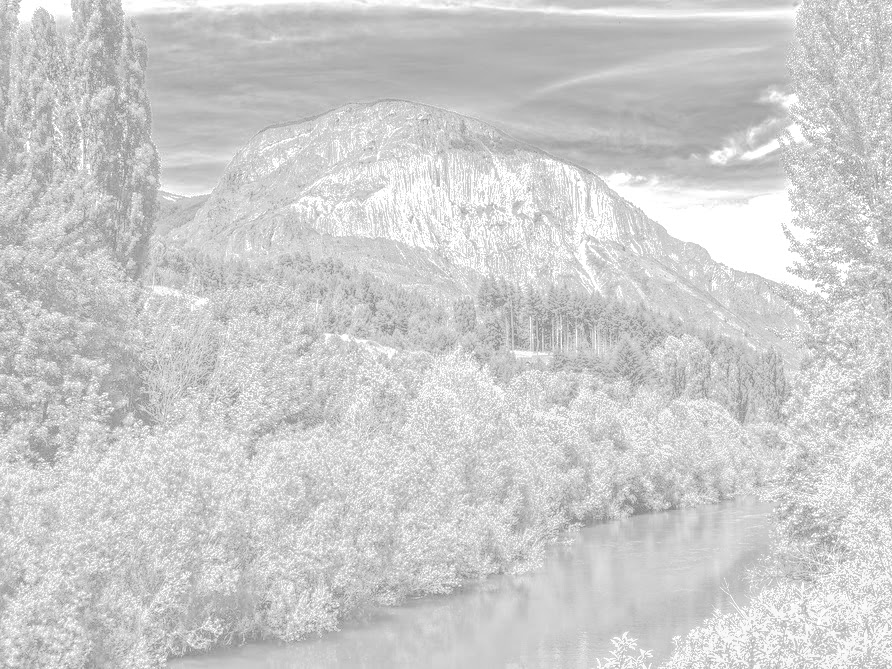
\includegraphics[width=\paperwidth]{aux/mackay.jpg}}}

	\setbeamercolor{background canvas}{bg=lgray}  % make background light gray

	\begin{frame}[plain,noframenumbering]
	    \titlepage
	\end{frame}
}
	\begin{frame}[plain,noframenumbering]{}
	\vspace*{2.3cm}
	\begin{center}
		\includegraphics[scale=.15]{aux/ukraine}
	\end{center}
\end{frame}
	%!TEX root = ../per_st_tk.tex

\begin{frame}{Today's goal}
	\pause
	Introduce \colorit{Steenrod barcodes}, a new family of computable invariants augmenting the traditional persistence pipeline.

	\pause\medskip
	\colorit{Example}
	\vskip-15pt
	\begin{figure}
		\centering
		\begin{subfigure}[b]{0.49\textwidth}
			\centering
			\includegraphics[width=\textwidth]{aux/s2_s4.pdf}
			\caption{$\mathrm C\,\Sigma(S^2 \vee S^4)$}
			\label{f:s2_s4}
		\end{subfigure}
		\begin{subfigure}[b]{0.49\textwidth}
			\centering
			\includegraphics[width=\textwidth]{aux/cp2.pdf}
			\caption{$\mathrm C\,\Sigma\,\bC\rP^2$}
			\label{f:cp2}
		\end{subfigure}
	\end{figure}
\end{frame}

\begin{frame}{Black box summary}
	\pause
	\colorit{\texttt{steenroder}} is a new ready-to-use \texttt{Python} tool computing extra barcodes.
	These occur in real-data, carry additional information and are stable.


\end{frame}

\begin{frame}{Viewpoint}
	\pause
	\colorit{A goal of algebraic topology} \\
	To construct invariants of spaces up to some notion of equivalence.

	\bigskip\pause
	\colorit{Today} \\
	CW complexes and homotopy equivalence.

	\bigskip\pause
	\colorit{A basic tension} \\
	Computability \colorit{vs} strength of invariants.

	\bigskip\pause
	\colorit{Example} \\
	Cohomology \colorit{vs} homotopy.

	\bigskip\pause
	\colorit{A more subtle one} \\
	Effectiveness \colorit{vs} functoriality of their constructions.

	\bigskip\pause
	\colorit{Example} \\
	Cohomology via chain complex \colorit{vs} maps to Eilenberg-Maclane spaces.
\end{frame}

\begin{frame}{Effectively defined cohomology}
	\pause
	\colorit{Poincar\'{e}'s idea} \\
	Break spaces into contractible combinatorial pieces: \\
	\begin{center}
		Simplices, cubes, ...
	\end{center}

	\pause
	\colorit{Kan--Quillen's idea} \\
	Replace spaces by functors with a geometric realization: \\
	\begin{center}
		Simplicial sets, cubical sets, ...
	\end{center}

	\pause
	\colorit{Compute cohomology} \\
	Using a chain complex assembled from the standard chain complexes: \\
	\begin{center}
		$\gchains(\gsimplex^n)$, $\gchains(\gcube^n)$, ...
	\end{center}

	\pause
	\colorit{Our goals (loosly stated)} \\
	Understand the diagonal map of these standard complexes better to
	present effective/local computations of finer invariants in cohomology.
\end{frame}
	%!TEX root = ../per_st_tk.tex

\begin{frame}{Shortcomings of Betti numbers}
	\pause
	Barcodes are based on the \colorit{Betti numbers} of spaces.

	\pause\bigskip
	But these \colorit{forget} much information.

	\pause\bigskip
	As graded \colorit{vector spaces}
	\[
	H^\bullet(\R \rP^2; \Ftwo) \cong H^\bullet(S^1 \vee S^2; \Ftwo).
	\]

	\pause
	Similarly, as graded \colorit{abelian groups}
	\[
	H^\bullet(\bC \rP^2; \Z) \cong H^\bullet(S^2 \vee S^4; \Z).
	\]

	\pause
	As graded \colorit{rings}
	\[
	H^\bullet(\Sigma(\bC \rP^2)) \cong H^\bullet(\Sigma(S^2 \vee S^4)),
	\]

	\pause\medskip
	As \colorit{modules} over the \colorit{Steenrod algebra}.
	\[
	H^\bullet(\Sigma(\bC \rP^2)) \not\cong H^\bullet(\Sigma(S^2 \vee S^4)),
	\]
\end{frame}

\begin{frame}{Intuition}
	\pause
	\begin{figure}
		\newcommand*{\xMin}{0}%
\newcommand*{\xMax}{4}%
\newcommand*{\yMin}{0}%
\newcommand*{\yMax}{4}%
\begin{center}
	\centering
	\begin{tikzpicture}[scale=.6]
		\draw[-{Latex[length=2mm]}] (-.5,\yMin)--(-.5,\yMax);
		\draw[-{Latex[length=2mm]}] (-.5,\yMin)--(-.5,\yMax-.5);
		\draw[-{Latex[length=2mm]}] (4.5,\yMin)--(4.5,\yMax);
		\draw[-{Latex[length=2mm]}] (4.5,\yMin)--(4.5,\yMax-.5);

		\draw[-{Latex[length=2mm]}] (\xMin, -.5)--(\xMax, -.5);
		\draw[-{Latex[length=2mm]}] (\xMin, 4.5)--(\xMax, 4.5);

		\draw (0,0)--(0,4)--(4,4)--(4,0)--(0,0);

		\draw[color=blue!50, very thick] (0,2) .. controls (1,2.5) and (3,1.5) .. (4,2);
		\draw[color=red!50, very thick] (0,1) .. controls (1,1.3) and (3,1) .. (4,1);

		\node at (2,5.3){Torus};
		\node at (2,-1.3){$\rank \Sq^1 = 0$};
	\end{tikzpicture}
	\hspace*{2cm}
	\begin{tikzpicture}[scale=.6]
		\draw[-{Latex[length=2mm]}] (-.5,\yMin)--(-.5,\yMax);
		\draw[-{Latex[length=2mm]}] (-.5,\yMin)--(-.5,\yMax-.5);
		\draw[-{Latex[length=2mm]}] (4.5,\yMax)--(4.5,\yMin);
		\draw[-{Latex[length=2mm]}] (4.5,\yMax)--(4.5,\yMin+.5);

		\draw[-{Latex[length=2mm]}] (\xMin, -.5)--(\xMax, -.5);
		\draw[-{Latex[length=2mm]}] (\xMin, 4.5)--(\xMax, 4.5);

		\draw (0,0)--(0,4)--(4,4)--(4,0)--(0,0);

		\draw[color=blue!50, very thick] (0,2) .. controls (1,2.5) and (3,1.5) .. (4,2);
		\draw[color=red!50, very thick] (0,1) .. controls (1,1) and (2,2.5) .. (4,3);

		\node at (2,5.3){Klein Bottle };
		\node at (2,-1.3){$\rank \Sq^1 = 1$};
	\end{tikzpicture}
%	\caption{Klein Bottle. $\rank \Sq^1 = 0$}
\end{center} % REMEMBER TO UNCOMMENT INSIDE
	\end{figure}

	\pause\bigskip
	\colorit{Question}: How to compute the product and Steenrod squares in practice?
\end{frame}
	%!TEX root = ../per_st_tk.tex

\begin{frame}{Steenrod construction}
	\pause
	Unlike the diagonal of spaces, chain approxs to it are \textbf{not} invariant under
	\[
	x \otimes y \stackrel{T}{\mapsto} y \otimes x.
	\]
	For example in $\gchains(\gcube) \to \gchains(\gcube) \ot \gchains(\gcube)$ we have
	\begin{center}
		\begin{tikzpicture}
		\draw[color=pblue, thick] (0,0)--(1,1);
		\draw[->] (1.25, .5) -- (1.75, .5);
		\end{tikzpicture}
		\begin{tikzpicture}
		\node at (-0.1, 1){};
		\draw[color=pblue, thick] (0,0)--(1,0)--(1,1);
		\draw (1,1)--(0,1)--(0,0);
		\end{tikzpicture}
	\end{center}

	\smallskip\pause
	To correct homotopically the breaking of this symmetry, Steenrod introduced \textbf{explicit} maps
	\[
	\Delta_i \colon \gchains(\gsimplex^n) \to \gchains(\gsimplex^n)^{\otimes 2}
	\quad \text{satisfying} \quad
	\partial \Delta_{i} = \big(1 \pm T \big) \Delta_{i-1},
	\]
	the cup-$i$ coproducts.

	\smallskip\pause
	These define the Steenrod squares as
	\[
	\begin{split}
		\Sq^k \colon H^\bullet(X; \Ftwo) &\to H^\bullet(X; \Ftwo) \\
		[\alpha] &\mapsto \big[ (\alpha \otimes \alpha) \Delta_i(-) \big]
	\end{split}
	\]
\end{frame}

\begin{frame}{Self-intersections}
	\pause
	Using Poincar\'e duality, squares measure \colorit{self-intersections} in certain cases.

	\pause\bigskip
	For example
	\begin{figure}
		\newcommand*{\xMin}{0}%
\newcommand*{\xMax}{4}%
\newcommand*{\yMin}{0}%
\newcommand*{\yMax}{4}%
\begin{center}
	\centering
	\begin{tikzpicture}[scale=.6]
		\draw[-{Latex[length=2mm]}] (-.5,\yMin)--(-.5,\yMax);
		\draw[-{Latex[length=2mm]}] (-.5,\yMin)--(-.5,\yMax-.5);
		\draw[-{Latex[length=2mm]}] (4.5,\yMin)--(4.5,\yMax);
		\draw[-{Latex[length=2mm]}] (4.5,\yMin)--(4.5,\yMax-.5);

		\draw[-{Latex[length=2mm]}] (\xMin, -.5)--(\xMax, -.5);
		\draw[-{Latex[length=2mm]}] (\xMin, 4.5)--(\xMax, 4.5);

		\draw (0,0)--(0,4)--(4,4)--(4,0)--(0,0);

		\draw[color=blue!50, very thick] (0,2) .. controls (1,2.5) and (3,1.5) .. (4,2);
		\draw[color=red!50, very thick] (0,1) .. controls (1,1.3) and (3,1) .. (4,1);

		\node at (2,5.3){Torus};
		\node at (2,-1.3){$\rank \Sq^1 = 0$};
	\end{tikzpicture}
	\hspace*{2cm}
	\begin{tikzpicture}[scale=.6]
		\draw[-{Latex[length=2mm]}] (-.5,\yMin)--(-.5,\yMax);
		\draw[-{Latex[length=2mm]}] (-.5,\yMin)--(-.5,\yMax-.5);
		\draw[-{Latex[length=2mm]}] (4.5,\yMax)--(4.5,\yMin);
		\draw[-{Latex[length=2mm]}] (4.5,\yMax)--(4.5,\yMin+.5);

		\draw[-{Latex[length=2mm]}] (\xMin, -.5)--(\xMax, -.5);
		\draw[-{Latex[length=2mm]}] (\xMin, 4.5)--(\xMax, 4.5);

		\draw (0,0)--(0,4)--(4,4)--(4,0)--(0,0);

		\draw[color=blue!50, very thick] (0,2) .. controls (1,2.5) and (3,1.5) .. (4,2);
		\draw[color=red!50, very thick] (0,1) .. controls (1,1) and (2,2.5) .. (4,3);

		\node at (2,5.3){Klein Bottle };
		\node at (2,-1.3){$\rank \Sq^1 = 1$};
	\end{tikzpicture}
%	\caption{Klein Bottle. $\rank \Sq^1 = 0$}
\end{center}
	\end{figure}
\end{frame}

\begin{frame}[fragile]{A new description of Steenrod's construction}
	\pause
	\colorit{Notation:}
	\[
	d_u[v_0, \dots, v_m] = [v_0, \dots, \widehat v_u, \dots, v_m]
	\]
	\pause\vspace*{-15pt}
	\[
	\rP_q^n = \set[\big]{U \subseteq \{0, \dots, n\} : \bars{U} = q}
	\]
	\pause\vspace*{-15pt}
	\[
	\forall \, U = \{u_1 < \dots < u_q\} \in \rP_q^n
	\]
	\pause\vspace*{-15pt}
	\[
	d_U = d_{u_1} \dotsm \, d_{u_q}
	\]
	\pause\vspace*{-15pt}
	\[
	U^\varepsilon = \big\{ u_i \in U \mid u_i + i \equiv \varepsilon \text{ mod } 2 \big\}
	\]

	\bigskip\pause
	\colorit{Definition (Med.)} \\
	For a basis element $x \in \gchains_m(\gsimplex^n, \Ftwo)$
	\vspace*{-5pt}
	\[
	\Delta_i(x) \ = \!\!\! \sum_{U \in \rP_{m-i}^n} \!\! d_{U^0}(x) \otimes d_{U^1}(x)
	\]
	\vspace*{-10pt}

	\pause
	\colorit{Example:}
	\vspace*{-5pt}
	\begin{align*}
	\Delta_0 [0,1,2] &=
	\Big( d_{12} \otimes \id + d_2 \otimes d_0 + \id \otimes d_{01} \Big) [0,1,2]^{\otimes 2} \\ &=
	[0] \otimes [0,1,2] + [0,1] \otimes [1,2] + [0,1,2] \otimes [2].
	\end{align*}
\end{frame}

\begin{frame}{Fast computation of Steenrod squares}
	\pause
	Comparing with SAGE: (algorithm based on EZ-AW contraction)

	\smallskip\pause
	\colorit{$\Sq^1$} on \colorit{$\Sigma^i\R P^2$} ($i^\th$ suspension of the real projective plane)

	\medskip
	\includegraphics[width=\textwidth]{aux/comp_sus_rp2.pdf}
\end{frame}

\begin{frame}{Steenrod squares for simplicial complexes}
	\begin{algorithm} [H]
	\KwIn{$A = \{a_1, \dots, a_m\} \subseteq X_n$}
	$B = \emptyset$ \\
	\ForAll{$a_i\ \mathrm{and}\ a_j\ \mathrm{with}\ i < j$}
	{
		$a_{ij} = a_i \cup a_j$ \\
		\If{$a_{ij} \in X_{n+k}$}
		{
			$\overline{a}_i = a_i \setminus a_j$\ ;\ \
			$\overline{a}_j = a_j \setminus a_i$\ ;\ \
			$\overline{a}_{ij} = \overline{a}_i \cup \overline{a}_j$ \\
			$index \colon \overline{a}_{ij} \to \{0,1\}$ \\
			\ForAll {$v \in \overline{a}_{ij}$}
			{
				$p = \mathrm{position\ of\ } v \mathrm{\ in\ } a_{ij}$\ ;\ \
				$\overline{p} = \mathrm{position\ of\ } v \mathrm{\ in\ } \overline{a}_{ij}$\\
				$index(v) = {p}\, +\, \overline{p}\ \ \mathrm{residue\ mod}\ 2$
			}
			\If{\hspace*{3pt}$index(\overline{a}_i) \xor index(\overline{a}_j)$ = $\{0,1\}$}
			{$B = B \xor \{a_{ij}\}$}
		}
	}
	\KwOut{$B$}
\end{algorithm}
\end{frame}

\begin{frame}[fragile]{Steenrod barcodes}
	\pause
	Given a filtered simplicial complex $X$
	\[
	X_0 \to X_1 \to \cdots \to X_n.
	\]

	\pause
	Cohomology induces a \colorit{persistent module}, its \colorit{barcode} is a summary of how Betti numbers are consecutively shared.\\

	\smallskip
	\phantom{A cohomology operation induces an endomorphism}
	\[
	\begin{tikzcd}[column sep = 15]
		H^\bullet(X_n; \Ftwo) \arrow[r] & \cdots \arrow[r] & H^\bullet(X_{n-1}; \Ftwo) \arrow[r] & H^\bullet(X_0; \Ftwo) \\
		\phantom{H^\bullet(X_n; \Ftwo)} \arrow[u, "\phantom{\Sq^k}", phantom] & \phantom{\cdots} & \phantom{H^\bullet(X_{n-1}; \Ftwo)} & \phantom{H^\bullet(X_0; \Ftwo)} \arrow[u, "\phantom{\Sq^k}", phantom] \phantom{.}
	\end{tikzcd}
	\]
\end{frame}

\begin{frame}[fragile]{Steenrod barcodes}
	Given a filtered simplicial complex $X$
	\[
	X_0 \to X_1 \to \cdots \to X_n.
	\]
	Cohomology induces a \colorit{persistent module}, its \colorit{barcode} is a summary of how Betti numbers are consecutively shared.

	\smallskip
	A cohomology operation induces an \colorit{endomorphism}
	\[
	\begin{tikzcd}[column sep = 15]
	H^\bullet(X_n; \Ftwo) \arrow[r] & \cdots \arrow[r] & H^\bullet(X_{n-1}; \Ftwo) \arrow[r] & H^\bullet(X_0; \Ftwo) \\
	H^\bullet(X_n; \Ftwo) \arrow[u, "\Sq^k"] \arrow[r] & \cdots \arrow[r] & H^\bullet(X_{n-1}; \Ftwo) \arrow[u, "\Sq^k"] \arrow[r] & H^\bullet(X_0; \Ftwo) \arrow[u, "\Sq^k"].
	\end{tikzcd}
	\]

	\pause
	\colorit{Definition (Lupo--Med.--Tauzin)} \\
	The \colorit{$\Sq^k$-barcode} of $X$ is defined as the barcode of $\mathrm{img}\ \Sq^k$.

	\pause\medskip
	\colorit{Theorem (Ling Zhou--Med.--M\'emoli)} \\
	These barcodes are stable.
\end{frame}

\begin{frame}{Example} \pause
	Filtrations of the cone on the suspension of $S^2 \vee S^4$ and $\bC \rP^2$.

	\pause
	\begin{figure}
		\centering
		\begin{subfigure}[b]{0.49\textwidth}
			\centering
			\includegraphics[width=\textwidth]{aux/s2_s4.pdf}
			\caption{$\mathrm C\,\Sigma(S^2 \vee S^4)$}
			\label{f:s2_s4}
		\end{subfigure}
		\begin{subfigure}[b]{0.49\textwidth}
			\centering
			\includegraphics[width=\textwidth]{aux/cp2.pdf}
			\caption{$\mathrm C\,\Sigma\,\bC\rP^2$}
			\label{f:cp2}
		\end{subfigure}
	\end{figure}
\end{frame}

\begin{frame}{Algorithm}
	\pause
	It has three steps:

	\begin{enumerate}
		\pause\bigskip
		\item Usual reduction applied to the anti-transposed boundary $M$ yielding
		\[
		R = M V
		\]
		where $R$ is reduced and $V$ is invertible.

		\pause\bigskip
		\item Read off cohomology representatives and apply the new $\Sq^k$ algorithm to create a matrix $Q^k$ with the resulting representatives.

		\pause\bigskip
		\item Using that $R$ is made of generating coboundaries, apply a reduction algorithm to $Q^k$ with respect to $R$ recording the rank of $Q_{\leq j}^k$.
	\end{enumerate}
\end{frame}

\begin{frame}{Third step}
	\begin{algorithm}[H]
	\KwIn{$R,\, Q^k$}
	Alive $= \{0, \dots, m\}$,
	Barcode $= \emptyset$ \\
	\For{$j = 0, \dots, m$}{
		$R_{\leq j} \mid Q^k_{\leq j} = \text{Reduce}\left( R_{\leq j} \mid Q^k_{\leq j} \right)$ \\
		\For{$i = 0, \dots, j$}{
			\If{$i \in \mathrm{Alive\ and\ } Q^k_i = 0$}{
				remove $i$ from Alive \\
				\If{$i <j $}{add $[m-j, m-i]$ to Barcode}
			}
		}
	}
	\For{$i \in \mathrm{Alive}$}{
		add $[-1, m-i]$ to Barcode
	}
	\KwOut{Barcode}
\end{algorithm}
\end{frame}

\begin{frame}{\texttt{steenroder}}
	\pause
	With \textit{U. Lupo} and \textit{G.~Tauzin}

	\begin{center}
		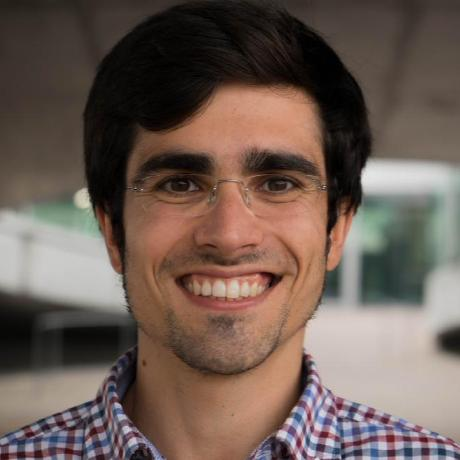
\includegraphics[scale=.2]{aux/umberto}
		\qquad
		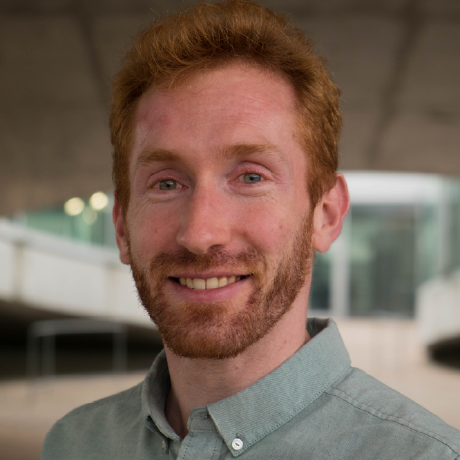
\includegraphics[scale=.2]{aux/guillaume}
	\end{center}

	from \colorit{\texttt{giotto-tda}}'s team we developed a Python package for this.

	\pause\smallskip
	It can easily installed via
	\begin{center}
		\texttt{python -m pip install -U steenroder}
	\end{center}

	and we accept contributions at
	\begin{center}
		\url{https://github.com/Steenroder/steenroder}
	\end{center}
\end{frame}

\begin{frame}{Space of conformations of $\mathrm{C_8H_{16}}$}
	\pause
	Points in $\R^{24}$ (positions of $8$ carbons in $\R^3$)

	\pause\smallskip
	Computing $\Sq^1$ barcode of a ``smooth component'' of this point cloud
	\smallskip
	\includegraphics[width=\textwidth]{aux/cyclo-octane_subsampled_absolute_barcodes.pdf}
	Consistent with a \colorit{Klein bottle} component.
\end{frame}

%\begin{frame}{Unicity of Steenrod's cup-$i$ construction}
%	\pause
%	\colorit{Theorem (Med.)} \\
%	All cup-$i$ constructions in the literature are equal up isomorphism:
%	\vskip -7.5pt
%	\[
%	\triangle \sim \triangle^\prime \iff \forall i \in \N, \ \triangle_i = \triangle_i^\prime \ \vee \, \triangle_i = T \triangle_i^\prime.
%	\]
%	\vskip -3pt
%	(Proven via an axiomatic characterization.)
%
%	\medskip\pause
%	\colorit{Theorem (Laplante-Anfossi--Med.--Vallette)} \\
%	Let $P \subset \R^n$ be an $n$-dim convex polytope.
%	A generic orthogonal ordered basis of $\R^n$ defines a cellular cup-$i$ construction $S^\infty \times P \to P \times P$.
%\end{frame}
	%!TEX root = ../per_st_tk.tex

\begin{frame}[fragile]{Future: Operations at odd primes}
	\pause
	Steenrod squares come from the symmetry of the \textbf{binary} diagonal.

	\medskip\pause
	Steenrod, and more generally May, also defined operations
	\[
	P_k \colon H^\bullet(X; \Fp) \to H^\bullet(X; \Fp)
	\]
	from the symmetry of diagonal $X \to X \times \dots \times X$.

	\medskip\pause
	\colorit{Note}: indirect group homology definition.
	No generalizations of cup-$i$.

	\bigskip\pause
	\colorit{Construction (Med.)} \\
	Explicit cup-$(p,i)$ coproducts defining these operations.

	\medskip\pause
	\colorit{Example} \\
	Using the computer algebra system \colorit{\texttt{ComCH}} we have $\Delta_{3,2}[0,1,2] = $

	\begin{verbatim}
		- [0,1][0,1,2][0,1] + [0,1,2][0,2][0,1] + [0,2][0,2][0,1,2]
		- [0,1,2][0,1,2][1] - [0,2][0,1,2][1,2] + [0,1,2][1,2][1,2]
		- [0,1][1,2][0,1,2] - [0,1,2][2][0,1,2] - [0][0,1,2][0,1,2]
	\end{verbatim}
\end{frame}

%\begin{frame}{A more abstract viewpoint}
%	\pause
%	Operads control algebraic structures.
%
%	\bigskip\pause
%	The operad $\cC om$ controls cocommutative and coassociative coalgebras.
%
%	\bigskip\pause
%	An $E_\infty$-operad is an $\sym$-cofibrant resolution of $\cC om$.
%
%	\bigskip\pause
%	Controls coalgebras cocomm. and coassoc. up to coherent homotopies.
%
%	\bigskip\pause
%	$E_\infty$-structures have a long history:
%	\smallskip\pause
%	\begin{itemize}
%		\item (co)homology operations,
%		\item recognition of infinite loop spaces,
%		\item algebraic models of the homotopy category.
%	\end{itemize}
%
%	\bigskip\pause
%	\colorit{Fact}:
%	Fully deriving its diagonal map, the chains of a space form an $E_\infty$-coalgebra.
%
%	\bigskip\pause
%	\colorit{Principle} (Quillen, Sullivan, Mandell, ...): \\
%	\textbf{All} homotopy information of spaces is in this algebraic model.
%
%	\bigskip\pause
%	\colorit{Question}: How explicit can this $E_\infty$-structure be made?
%\end{frame}
%
%\begin{frame}{Explicit $E_\infty$-structure on (co)chains}
%	\pause
%	\colorit{Theorem (Med.)} \\
%	The collection of maps $\gchains(\gsimplex^n) \to \gchains(\gsimplex^n)^{\otimes r}$ obtained from compositions of
%	\begin{align*}
%		\Delta &\colon \gchains(\gsimplex^n) \to \gchains(\gsimplex^n)^{\otimes 2}
%		\qquad \text{(AW diagonal)} \\
%		\ast &\colon \gchains(\gsimplex^n)^{\otimes 2} \to \gchains(\gsimplex^n)
%		\qquad \text{(Join map)}
%	\end{align*}
%	defines an $E_\infty$-coalgebra on simplicial chains.
%
%	\bigskip\pause
%	\colorit{Join map} \\
%	\qquad\qquad \scalebox{0.7}{\begin{tikzpicture}[scale=.6]
\coordinate (A) at (210:2);
\coordinate (B) at (-30:2);
\coordinate (C) at (90:2);

\draw[draw=black] (A) -- (B) -- (C) -- (A);

\node[circle,fill=blue, opacity=.9, inner sep=0pt,minimum size=5pt, label=left:{0}] (a) at (A) {};
\node[circle,fill=black,inner sep=0pt,minimum size=3pt, label=right:{$1$}] (a) at (B) {};
\node[circle,fill=black,inner sep=0pt,minimum size=3pt, label=right:{$2$}] (a) at (C) {};

\node[scale=1.5] at (3.5,0.5) {$\ast$};
\end{tikzpicture}
\begin{tikzpicture}[scale=.6]
\coordinate (A) at (210:2);
\coordinate (B) at (-30:2);
\coordinate (C) at (90:2);

\draw[draw=blue,  ultra thick, draw opacity=.7] (B) -- (C);
\draw[draw=black] (C) -- (A);
\draw[draw=black] (A) -- (B);

\node[circle,fill=black,inner sep=0pt,minimum size=3pt, label=left:{$0$}] (a) at (A) {};
\node[circle,fill=black,inner sep=0pt,minimum size=3pt, label=right:{$1$}] (a) at (B) {};
\node[circle,fill=black,inner sep=0pt,minimum size=3pt, label=right:{$2$}] (a) at (C) {};

\node[scale=1.5] at (3.5,.5) {=};
\end{tikzpicture}
\begin{tikzpicture}[scale=.6]
\coordinate (A) at (210:2);
\coordinate (B) at (-30:2);
\coordinate (C) at (90:2);

\draw[draw=black] (A) -- (B) -- (C) -- (A);

\node[circle,fill=black,inner sep=0pt,minimum size=3pt, label=left:{$0$}] (a) at (A) {};
\node[circle,fill=black,inner sep=0pt,minimum size=3pt, label=right:{$1$}] (a) at (B) {};
\node[circle,fill=black,inner sep=0pt,minimum size=3pt, label=right:{$2$}] (a) at (C) {};

\draw[draw, fill=blue, opacity=.7] (A) -- (B) -- (C) -- (A);
\end{tikzpicture}}
%
%	\bigskip\pause
%	\colorit{Other versions} \\
%	\colorit{1)} Cubical (Kaufmann--Med.) \\
%	\colorit{2)} Multisimplicial (Med.--Pizzi--Salvatore).
%\end{frame}

	%!TEX root = ../per_st_tk.tex

\begin{frame}[fragile]{Future: Operations at odd primes}
	\pause
	Steenrod squares come from the symmetry of the \textbf{binary} diagonal.

	\medskip\pause
	Steenrod, and more generally May, also defined operations
	\[
	P_k \colon H^\bullet(X; \Fp) \to H^\bullet(X; \Fp)
	\]
	from the symmetry of diagonal $X \to X \times \dots \times X$.

	\medskip\pause
	\colorit{Note}: indirect group homology definition.
	No generalizations of cup-$i$.

	\bigskip\pause
	\colorit{Construction (Med.)} \\
	Explicit cup-$(p,i)$ coproducts defining these operations.

	\medskip\pause
	\colorit{Example} \\
	Using the computer algebra system \colorit{\texttt{ComCH}} we have $\Delta_{3,2}[0,1,2] = $

	\begin{verbatim}
		- [0,1][0,1,2][0,1] + [0,1,2][0,2][0,1] + [0,2][0,2][0,1,2]
		- [0,1,2][0,1,2][1] - [0,2][0,1,2][1,2] + [0,1,2][1,2][1,2]
		- [0,1][1,2][0,1,2] - [0,1,2][2][0,1,2] - [0][0,1,2][0,1,2]
	\end{verbatim}
\end{frame}
	%!TEX root = ../per_st_tk.tex

{
	\usebackgroundtemplate{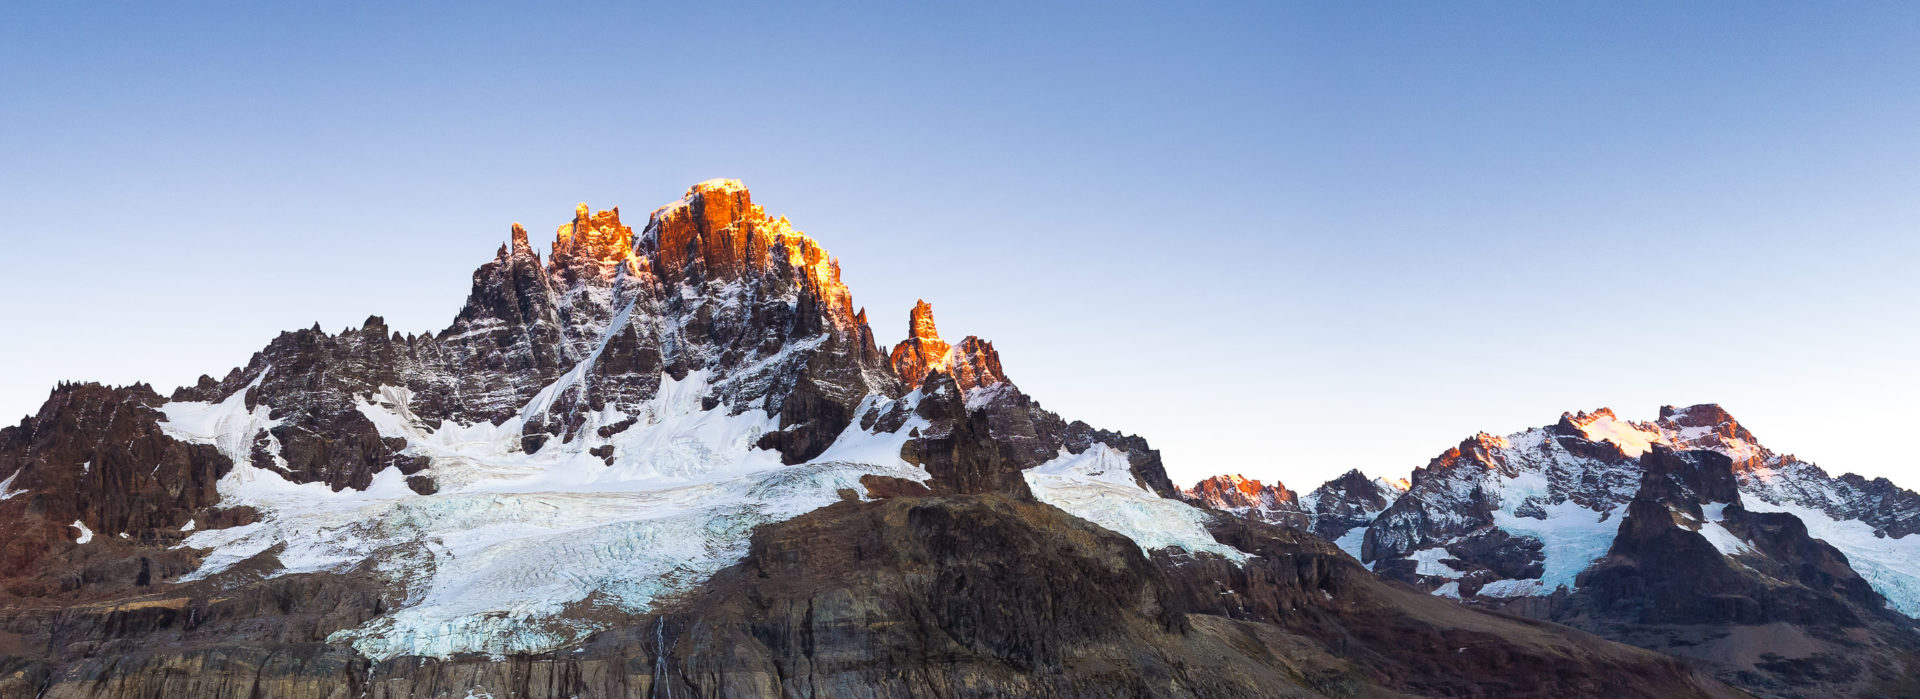
\includegraphics[width=\paperwidth]{aux/castillo.jpg}}%
	\begin{frame}
		\vskip 5cm
		\begin{center}
			\colorit{\Huge Thank you!}
		\end{center}

	\bigskip

	\footnotesize
	\colorit{1.} Medina-Mardones, Anibal M. ``New formulas for cup-$i$ products and fast computation of Steenrod squares." Computational Geometry 109 (2023).

	\medskip
	\colorit{2.} Umberto Lupo, Anibal M. Medina-Mardones, and Guillaume Tauzin. ``Persistence Steenrod modules." Journal of Applied and Computational Topology (2022).
	\end{frame}
}
\end{document}
